\documentclass[french,10pt]{article}
\usepackage[T1]{fontenc}
\usepackage[utf8]{inputenc}
\usepackage{lmodern}
\usepackage[a4paper,top=1.0cm, left=1.0cm, right = 1.0cm, bottom = 1.2cm]{geometry}
\usepackage{amsmath}
\usepackage{tikz}
\usepackage{pgfplots}
\usepackage{subfig}
\usepackage{placeins}
\usepackage{enumerate}

\usetikzlibrary{calc}
\usetikzlibrary{decorations.markings}
\usetikzlibrary{angles,quotes} % for pic
\usetikzlibrary{arrows.meta} % for arrow size
\usetikzlibrary{bending} % for arrow head angle
\usetikzlibrary{decorations.pathmorphing} % for decorate random steps
\tikzset{>=latex} % for LaTeX arrow head

\def\spaceans{\underline{\hspace{1cm}}}
\def\spaceTF{$\big(\quad\big)$}

%%\usepackage[usenames, dvipsnames]{xcolor}
%\usepackage[utf8x]{inputenc}
\usepackage[T1]{fontenc}
\usepackage{tikz}
\usepackage{pgfplots}
\usetikzlibrary{calc,arrows,fadings,decorations.pathreplacing,decorations.markings,patterns,shapes.geometric}
\usepackage{calc}	    	% Faire des calculs sur les longueurs.
\usepackage{ifthen}		
\usepackage{fp}
\usepackage{verbatim}
\usepackage[active,tightpage]{preview}
%\PreviewEnvironment{tikzpicture}
\setlength\PreviewBorder{5pt}

%------ mes couleurs -------
\definecolor{fond}{rgb}{1,0.9,0.75}
\definecolor{filet}{rgb}{1,0.6,0}
\definecolor{monOrange}{RGB}{255,157,0}
\definecolor{monBleu}{rgb}{0.2,0.4,0.6}
% \definecolor{monBleu}{RGB}{54,134,193}
\definecolor{monCyan}{RGB}{74,181,247}
\definecolor{monGris}{RGB}{100,100,100}

%------ styles tikz ---------------
\colorlet{darkblue}{blue!50!black} 
\tikzset{>=stealth,inner sep=0pt, outer sep=2pt,}
\tikzset{tiret/.style={gray,dashed}}
\tikzset{doublefleche/.style={|<->|,>=stealth,thin}}
\tikzset{titre/.style={inner sep=0pt, outer sep=0pt,above right,text justified,fill=orange!50}}
\tikzset{bloc/.style={rounded corners=4pt,color=white,ball color=lightgray,smooth}}
\tikzset{force/.style={->,ultra thick,rounded corners=4pt,color=monBleu,smooth,line cap=round}}
\tikzset{vecteur/.style={->,thick,color=black,smooth}}
\tikzset{verre/.style={draw=SkyBlue,fill=SkyBlue!30}}
\tikzset{axis/.style={thin,gray}}
\tikzset{figure/.style={thick,color=#1,fill=purple, opacity=0.5}}
\tikzset{ressort/.style={very thick,black,smooth}}
\tikzset{eau/.style={draw=black,fill=blue,opacity=0.5}}
\tikzset{rayon/.style={draw=red!66,thick,line join=round}}
%-----------------------------------

%-------- patatoide ----------
\newcommand{\patate}[1][fill=white] 
{\draw [#1][preaction={fill=white}] (0,0) .. controls +(0.1,0.2) and +(0.3,0.3) .. (1,0) .. controls +(-0.3,-0.3) and +(-0.05,0.15) .. (1,-1) .. controls +(0.2,-0.6) and +(0.1,-0.2) .. (0,-1) .. controls +(-0.1,0.15) and +(-0.2,-0.4) .. (0,0);}
%------ aimant -------
\newcommand{\aimant}[1][ultra thick]{
\draw[fill, color=red,#1] (0,0.2) rectangle(1,-0.2) node[color=white,midway]{\tiny S};
\draw[fill, color=black,#1] (1,0.2) rectangle(2,-0.2) node[color=white,midway]{\tiny N};}

% ------ \arcdecercle{}--- longueur d'arc
\newlength{\longueurarcdecercle}
\newcommand{\arcdecercle}[1]{\ensuremath{%
    \settowidth{\longueurarcdecercle}{\ensuremath{#1}}%
    \overset{%
        \mbox{%
                \resizebox{\longueurarcdecercle-2pt}{3pt}{%
                        \rotatebox{90}{\ensuremath{\hskip-1pt)}}%
                }%
        }%
    }{\text{#1}}%
}}

% commande \resistanceH{option}{nom}  : résistance de longueur unité, centrée en (0,0).
\newcommand{\resistanceH}[2]
{
\draw[#1,fill=white] (-0.5,3pt)--++(1,0)--++(0,-6pt)--++(-1,0)--cycle;
\draw[#1] (0,0) node[above=3pt]{\footnotesize #2};
}
% commande \resistanceV{option}{nom}  : résistance de longueur unité, centrée en (0,0).
\newcommand{\resistanceV}[2]
{
\draw[#1,fill=white] (-3pt,0.5)--++(0,-1)--++(6pt,0)--++(0,1)--cycle;
\draw[#1] (0,0) node[left=3pt]{\footnotesize #2};
}
% \condoH{options}{nom}{valeur} : condensateur horizontal de longueur unité, centrée en (0,0)
\newcommand{\condoH}[3]%
{
\fill[#1,white] (-3pt,-0.5)rectangle(3pt,0.5);
\draw[#1,ultra thick] (-3pt,-0.3)--++(0,.6);
\draw[#1,ultra thick] (3pt,-0.3)--++(0,.6);
\draw[#1] (0,-0.3) node[below]{\footnotesize #3};
\draw[#1] (0,0.3) node[above]{\footnotesize#2};
}

% \condoV{options}{nom}{valeur} : condensateur vertical de longueur unité, centrée en (0,0)
\newcommand{\condoV}[3]%
{ 
\fill[#1,white] (-0.5,-3pt)rectangle(0.5,3pt);
\draw[#1,ultra thick] (-0.3,-3pt)--++(.6,0);
\draw[#1,ultra thick] (-0.3,3pt)--++(.6,0);
\draw[#1] (0.3,0) node[right]{\footnotesize #3};
\draw[#1] (-0.3,0) node[left]{\footnotesize #2};
}

% \bobineH{options}{nom}{valeur} : bobine horizontal de longueur unité, centrée en (0,0)
\newcommand{\bobineH}[3]%
{
\fill[#1,white] (-5mm,-3pt) rectangle (5mm,3pt);
\draw[#1,fill=white,decoration={coil,aspect=0.5,segment length=2mm,amplitude=2mm},decorate] (-0.5,0)--++(1,0)node[midway,above=6pt]{\footnotesize #2} node[midway,below=5pt]{\footnotesize #3};
}



     


\definecolor{monOrange}{RGB}{255,157,0}
\tikzset{vecteur/.style={->,thick,color=black,smooth}}
\tikzset{force/.style={->,ultra thick,rounded corners=4pt,color=monBleu,smooth,line cap=round}}
\definecolor{monBleu}{rgb}{0.2,0.4,0.6}


\title{ \large
Faculté de Sciences et Technologie - UPEC \\
Préparation $1^{er}$ Contrôle Continu de Mécanique du Point 2 (07/03/2024)\\ }
\author{Responsable TD: Felipe FIGUEREDO ROCHA \\ \texttt{felipe.figueredo-rocha@u-pec.fr}}

\date{}
\begin{document}
	
	\maketitle

	\subsection*{Diagnostique}
	\subsection*{Rappels}
	\begin{itemize}
		\item Dérivé d'un fonction composé: $(f \circ g)'(x) = (f' \circ g)(x) g'(x)$.
		\item Produit scalaire en deux dimensions : $\vec{a} \cdot \vec{b} = a_x b_x + a_y b_y = \|a\| \|b\| \cos{\theta}$, où $\theta$ est l'angle entre $\vec{a}$ et $\vec{b}$.
		\item Quelques relations en repère polaire avec l'angle $\theta$ mesuré par rapport $\Vec{u}_x$ (ci-dessous dépendance explicite du temps omis, $r=r(t) , \theta=\theta(t), \Vec{u}_r = \Vec{u}_r(t), \Vec{u}_{\theta} = \Vec{u}_{\theta}(t)$):
		\begin{align*}
			\Vec{u}_r &= \cos{\theta} \Vec{u}_x + \sin{\theta} \Vec{u}_y, \quad \Vec{u}_{\theta} = -\sin{\theta} \Vec{u}_x + \cos{\theta} \Vec{u}_y, \quad, \\
			\dot{\Vec{u}}_r &= \dot{\theta} \Vec{u}_{\theta}, \quad  \dot{\Vec{u}}_{\theta} = -\dot{\theta} \Vec{u}_{r}, \\
			\Vec{v}(t) &= \dot{r} \Vec{u}_r + r \dot{\theta} \Vec{u}_{\theta}, \quad
			\Vec{a}(t) = (\ddot{r} - r\dot{\theta}^2) \Vec{u}_r + (2 \dot{r} \dot{\theta} + r \ddot{\theta}) \Vec{u}_{\theta}
		\end{align*}
	\item Règle de la main droite (Figure \ref{fig:regledelamaindroite}).
	\begin{figure}[h!]
		\centering
		\includegraphics[width=0.35\linewidth]{regle_de_la_main_droite}
		\caption{Schéma de la règle de main droite.}
		\label{fig:regledelamaindroite}
	\end{figure}
	 
	\end{itemize}

	\FloatBarrier

	\subsection*{Q1 Produit Vectoriel}
	Dans la Figure \ref{fig:vector_product_in_space}, le vecteur $\vec{B}$ est aligné vers $\vec{u}_y$ et $\vec{A}$ se trouve dans le plan formé par $\vec{u}_x$ et $\vec{u}_y$. 
	\begin{enumerate}[a)]
	\item Dessiner le vecteur $\vec{C} = \vec{A}  \wedge \vec{B}$ dans la Figure \ref{fig:vector_product_in_space} (la taille de la flèche n'est pas important).
	\item Calculer $\|\vec{C}\|$ en sachant que $\|\vec{B}\| = 1$ et en fonction des constants de la figure?
	\item Calculer $\vec{A}$ en fonction de $h$ et $\theta$.
	\item Calculer $\vec{C}$ avec l'expression du produit vectoriel et vérifier que $\|\vec{C}\|$ correspond au résultat trouvé dans b).
	\item En prenant $\vec{D} = D_x \vec{u}_x$, calculer la valeur de $D_x$ tel que $\vec{B} \wedge \vec{D} = -2 \vec{C}$.
	\item Dans le plan x-z de la Figure \ref{fig:plan_xz}, dessiner les vecteurs $\vec{u}_y$, $\vec{B}$, $\vec{C}$, $\vec{D}$ et $\vec{B} \wedge \vec{D}$. Utilisez respectivement les notations $\otimes$ ou $\odot$ pour représenter un vecteur qui rentre ou qui sort du plan de feuille.
	\end{enumerate}
	
	\begin{figure}
		\centering
	\begin{tikzpicture} [scale=1.5,x={(-0.353cm,-0.353cm)}, y={(1cm,0cm)}, z={(0cm,1cm)}]
		\coordinate (O) at (0, 0, 0);
		\coordinate (A) at (1,1,0);
		\coordinate (B) at (3,2,0);
		\coordinate (C) at (3,4,0);
		\coordinate (D) at (1,3,0);
		\coordinate (E) at (1,2,0);
		%axes et vecteurs unitaires  et définition de x,y,z
		\draw[gray,thin] (O) -- +(3, 0,   0) ;
		\draw[gray,thin] (O) -- +(0,  3.5, 0) ;
		\draw[gray,thin] (O) -- +(0,  0, 2) ;
		\draw[vecteur] (O)-- ++(1,0,0)node[midway,left=5pt]{$\overrightarrow{{u}_{x}}$};
		\draw[vecteur] (O)-- ++(0,1,0)node[above]{$\overrightarrow{{u}_{y}}$};
		\draw[vecteur] (O)-- ++(0,0,1)node[midway,left]{$\overrightarrow{{u}_{z}}$};
		\fill[black](O)--++(.3,0,0)--(.3,.2,0)--(0,.2,0)--cycle;
		% parallelogramme
		\fill[monOrange](A)--(B)--(C)--(D);
		\draw[gray,dashed](B)--(C)--(D);
		\draw[thin](B)--(E)node[midway,right]{$h$};
		\draw[thin](1.5,1.25,0) to[bend right] (1,1.5,0);
		\draw (1.75,1.75,0)node{$\theta$};
		\fill[black](E)--++(.3,0,0)--++(0,.2,0)--++(-.3,0,0)--cycle;
		% vecteurs
		\draw[force] (A)--(B)node[midway,left]{$\overrightarrow{A}$};
		\draw[force] (A)--(D)node[right]{$\overrightarrow{B}$};
		%\draw[force] (A)--++(0,0,2)node[right]{$\overrightarrow{C}$};
	\end{tikzpicture} 
		\caption{}
		\label{fig:vector_product_in_space}
	\end{figure}
	
	\begin{figure}
	\centering	
	\begin{tikzpicture}
		\coordinate (O) at (0,0);
		\coordinate (X) at (1.8,0);
		\coordinate (Y) at (0,1.8);
		\coordinate (R) at (-0.6, 1.5);
		\coordinate (T) at (1.5, 0.6);	
		\draw[very thick,->] node[below left]{$O$} (O)--(X) node[right]{$\vec{u}_{x}$};
		\draw[very thick,->](O)--(Y) node[right]{$\vec{u}_{z}$};
	\end{tikzpicture}
		\caption{}
		\label{fig:plan_xz}
	\end{figure}
	
	
	\subsection*{Q1 (14 pts) : skateur dans un half-pipe (analogue pendule)}
	Un skateur de masse $m$ est sur un half-pipe semi-circulaire (moitié d'un cercle) de rayon $R$. On va considérer le skateur comme une particule M qui ne décolle jamais du half-pipe, c'est-à-dire, il sera toujours à une distance $R$ de l'origine $O$. On repère la position du skateur par l'angle $\theta$ qu'il fait avec la vertical descendent depuis $O$. La norme de l'accéleration de la pesanteur est dénoté $g$ (le vecteur $\Vec{g}$ pointe vers le bas). On va étudier ce mouvement en repère polaire.
	\begin{enumerate}
	\item(0,5 pts) Complétez la Figure 1 ci-dessous en plaçant $\theta$, $\Vec{u}_x$, $\Vec{u}_y$, $\Vec{u}_r$, $\Vec{u}_\theta$ selon la convention usuelle (voir rappel si besoin et notez qu'il y a de flèches en plus).
	\textbf{réponse} En bleu:
	\begin{figure}
		\centering
		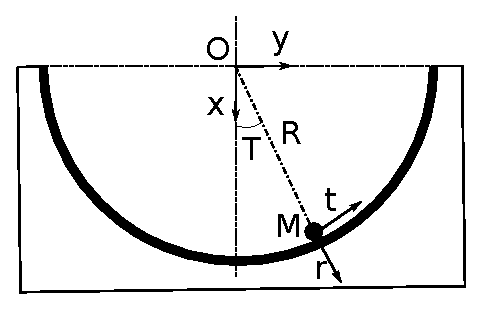
\includegraphics[width=0.5\linewidth]{halfpipe}
		\caption{}
		\label{fig:halfpipe}
	\end{figure}

 	\FloatBarrier
	
	
	\item (1 pts) Faire un bilan de forces (sans frottement) appliquer sur la particule $M$ et donner les expressions de toutes les forces en repère polaire (n'oubliez pas de dessiner ces vecteurs). \\
	\textbf{réponse}: $\boxed{\vec{P} = mg( -\sin \theta \vec{u}_{\theta} + \cos \theta \vec{u}_r)}$ et $\boxed{\vec{R}_N = -R_N\vec{u}_r}$ (les vecteurs de base peuvent être placés n'importe où).
	\begin{center}
		\begin{tikzpicture}
			\coordinate (G) at (0,-4.5);
			\coordinate (T) at (0,0);
			\coordinate (M) at (1,-3);
			\coordinate (Meps) at (1+0.03,-3-0.09);
			\coordinate (O) at (0,0);
			\coordinate (Ort) at (0.9,0.3);
			\coordinate (Ord) at (0.3,-0.9);
			\coordinate (Md) at (1,-4.2);
			\coordinate (Mrd) at (1.25,-3.75);	
			\fill (M) circle[radius=4pt]  node[left]{$m,M$};	
			\draw[very thick,->](O)--(Ort) node[right]{$\vec{u}_{\theta}$};
			\draw[very thick,->](O)--(Ord) node[right]{$\vec{u}_{r}$};
			\draw[very thick,->](M)--(Md) node[right]{$\vec{P} = m \vec{g}$};
			\draw[very thick,<-](Meps)--(Mrd) node[above right]{$\vec{R}$};
			\draw[dashed] (G)--(T);
			\draw[dashed](M)--(O) node[left]{$O$};
			\pic[draw, ->, "$\theta$", angle radius=50, angle eccentricity=1.2] {angle = G--O--M};
		\end{tikzpicture}
	\end{center}
	\item (1 pts) Donner les expressions simplifiés pour ce type de mouvement pour les vecteurs vitesse $\Vec{v}$ et accélération $\Vec{a}$ en repère polaire (voir rappel). \\
	\textbf{réponse}: Comme $r = R = cte$, donc $\ddot{r} = \dot{r} = 0$. On a donc:
	$$\boxed{\Vec{v}(t) = R \dot{\theta} \Vec{u}_{\theta}, \quad
	\Vec{a}(t) = - R\dot{\theta}^2 \Vec{u}_r + R \ddot{\theta} \Vec{u}_{\theta}}$$
	


	
	\item (1 pts) Appliquer le principe fondamentale de la dynamique (PFD) et les projeter sur l'axe $\Vec{u}_{\theta}$ et $\Vec{u}_{r}$. \\
	\textbf{réponse}: du PFD, on a $m \vec{a} = \sum \vec{F} = \vec{P} + \vec{R}_N$. En composants on a
	\begin{align*}
		\boxed{
	\begin{cases}
			-mg \sin \theta  = m R \ddot{\theta} \quad (\text{sur} \; \vec{u}_{\theta} ),\\
			 mg \cos \theta - R_N = - m R\dot{\theta}^2 \quad (\text{sur} \; \vec{u}_{r} )
	\end{cases}
	}
	\end{align*}

	\item (1 pts) En utilisant le PFD sur $\Vec{u}_{\theta}$, déduire l'équation différentiel qui gouverne ce mouvement en utilisant l'approximation $\sin \theta \approx \theta$ pour des petites oscillations. \\
	\textbf{réponse}: $\boxed{R \ddot{\theta} + g \theta = 0}$.
	\item (1 pts) Vérifiez qu'une solution du type $\theta(t) = A \sin{\omega t}$ peut satisfaire l'équation précédent. Donner aussi l'expression pour $\omega$ en fonction de $g$ et $R$. \\
	\textbf{réponse}: En replaçant $\ddot{\theta} = -\omega^2 A \sin{\omega t}$ sur l'ED on a	
	\begin{align*}
    (-\omega^2 R + g) A \sin{\omega t}  = 0.
	\end{align*}	
	Cette équation est vrai si : $A = 0$, $\forall \omega, t$ (pas très amusant) et $\boxed{\omega = \sqrt{g/R}}, \forall A, t$.
	\item (1 pts) Dans l'instant initial le skateur est au tout au fond du half-pipe, avec $\theta(0) = 0$, et il imprime une vitesse angulaire (par exemple en s'autopropulsant avec ces pieds) de sorte que $\dot{\theta}(0) = \dot{\theta}_0$. Déterminez la constant $A$ en fonction de $\dot{\theta}_0$ et $\omega$. Qu'est-ce que représente $A$ et donner sa dimension. 
	
	\textbf{réponse}: D'abord on vérifie $\theta(0) = A \sin{\omega \times 0} = 0$, ce qui correspond à la condition initiale. Par contre cette condition ne nous permet pas de trouver $A$. Prenons sa dérivé dans l'instant $t=0$: $\dot{\theta}(0) = \omega A \cos{\omega \times 0} = \omega A$. De la condition initiale de la vitesse angulaire, on trouve que $\omega A = \dot{\theta}_0 \Rightarrow \boxed{A = \frac{\dot{\theta}_0}{\omega}}$. Finalement $A$ représente l'angle maximale qui la particule $M$ atteint, ce qui est une grandeur sans dimension (ou égale $1$). Cette interprétation vient directement de l'expression de $\theta(t)$. Alternativement on trouve que $A$ est sans dimension car $\dot{\theta}_0$ et $\omega$ ont les mêmes dimensions.
	\item (0,5 pts) Ce mouvement circulaire est-il uniforme ou non-uniforme? pourquoi? \\
	\textbf{réponse}: Non-uniforme car la vitesse angulaire n'est pas constant. \footnote{Le mouvement est accéléré ($\vec{a} \neq \vec{0}$) même pour le cas uniforme (vitesse angulaire constant, c'est-à-dire, $\ddot{\theta} = 0$).}.   
	\item (1 pts) Pour le cas particulier de $R = 10 \rm m$, $g = 10 \rm{m/s^2}$, $\dot{\theta}_0 = 5\times 10^{-2} \rm{rad/s}$, calculer $\omega$ et $A$. \\
	\textbf{réponse}: $ \omega = \sqrt{10/10} = \boxed{1 \, \textrm{rad/s} }$ et $A = 5 \times 10^{-2}/1 = \boxed{5\times 10^{-1} \textrm{rad}}$. Obs: $\rm rad$ est optionnel.
	
	\item (1 pts) Pour ce cas particulier, tracer $\theta(t)$ pour $t \in [0 \rm s,T]$, où $T$ est temps nécessaire pour que la fonction sinus complète son cycle. N'oubliez pas de calculer $T$ (en fonction de $\pi$) et d'écrire la valeur de $T$ et $A$ sur le dessin. \\
	\textbf{réponse:} $T = 2\pi/\omega = 2\pi/ 1 = 2\pi \rm s$. \\
	\begin{tikzpicture}
		\begin{axis}[
			%		xmin=-0.2, xmax=4, ymin=-0.2, ymax=3, 
			axis x line=middle, 
			axis y line=middle, 
			xlabel = {$t$},
			ylabel = {$\theta(t)$},
			ymajorgrids=true,
			xmajorgrids=true,
			grid style=dashed,
			xmin=-0.2,xmax=4.5,
			ymin=-1.5,ymax=1.5,
			xtick={1,2,3,4},
			xticklabels={$T/4$,$T/2$,$3T/4$,$\qquad \quad T = 2\pi \rm s$},
			ytick={-1,0,1},
			yticklabels={$-A = - 5\times 10^{-2}$, $0$, $A = 5\times 10^{-2}$}
			]	
			\addplot[very thick, domain=0:4]{sin(90*x)};
		\end{axis}
	\end{tikzpicture}

	\item (1 pts) Donner l'expression d'énérgie cinétique générique en fonction de $R$, $m$ et $\dot{\theta}$ (utilisez la formule de vitesse du l'exercise 3). \\
	\textbf{réponse:} $E_c = \frac{1}{2} m (R \dot{\theta}\vec{u}_{\theta}) \cdot (R \dot{\theta} \vec{u}_{\theta}) = \boxed{\frac{1}{2} m R^2 \dot{\theta}^2}$.
	\item (1 pts) Pour le cas particulier l'exercise 9 et pour $m=80 \rm kg$, calculer l'énergie cinétique du skateur de masse  à l'instant $t=0 \rm s$. 
	\textbf{réponse:} $E_c^0 = E_c(t=0) = \frac{1}{2} m R^2 \dot{\theta}_0^2 =  \frac{1}{2} \times 80 \times 10^2 \times (5\times 10^{-2})^2 = 40 \times 25 \times 10^{-2} = \boxed{10 \rm J}$.
	\item (1 pts) Donner l'expression du travail $W_{0\to f}(\vec{P})$ réalisé par la force de poids entre $\theta_0 = 0 \, \rm rad$ et $\theta_f$, en fonction des valeurs génériques de $m, g, \theta_f$, et $R$. \\
	\textbf{réponse:} Comme $d \vec{OM} = R d\theta \vec{u}_{\theta}$, on prend en considération juste la composant $\theta$ de la force poids. On a donc $W_{0\to f}(\vec{P}) = \displaystyle \int_{0}^{\theta_f} -mg \sin \theta R d \theta = mg R \cos \theta \big|_{0}^{\theta_f} = \boxed{m g R (\cos \theta_f - 1)}$.
	\item (1 pts) En utilisant le théorème d'énergie cinétique, donner l'expression pour $\dot{\theta}_{0}$ nécessaire pour que le skateur arrive jusqu'au bord supérieur du half-pipe (à $\theta_f = \pi/2$) mais sans le dépasser. \\
	\textbf{réponse:} Sachant que $\vec{R}_N \perp d \vec{OM}$ son travail est nulle. Comme $M$ ne peut pas dépasser le bord supérieur, sa vitesse doit être nulle à $\theta_f = \pi/2$, donc $E_c^f = 0 \rm J$. Dans l'instant initiale $E^0_c = \frac{1}{2} m R^2 \dot{\theta}_0^2$. Finalement, du TEC, viens que \footnote{Pas besoin de résoudre le résultat finale.}
	\begin{align*}
	E_c^f - E_c^0 = W_{0\to f}(\vec{P}) \Rightarrow 0 - \frac{1}{2} m R^2 \dot{\theta}_0^2 = m g R (\cos{\pi/2} - 1) \\
	- \frac{1}{2} m R^2 \dot{\theta}_0^2 = - m g R  \Rightarrow \boxed{\dot{\theta}_0 = \sqrt{\frac{2\times g}{R}}}.
 	\end{align*}
	\item (1 pts) Maintenant, une force de frottement constant est présent $\vec{f} = -f \vec{u}_{\theta}$ (en supposant $\dot{\theta}_{0}$ > 0), donner une expression $\dot{\theta}_{0}$ sous les mêmes conditions du problème précédent. \\
	\textbf{réponse:} Le travail de la force de frottement est $W_{0\to f}(\vec{f}) = \int_{0}^{\pi/2} -f R d\theta = -fR\pi/2$. Finalement, du TEC, viens que
	\begin{align*}
		E_c^f - E_c^0 = W_{0\to f}(\vec{P}) + W_{0\to f}(\vec{f})\Rightarrow - \frac{1}{2} m R^2 \dot{\theta}_0^2 = -m g R - f R (\pi/2) \\ \Rightarrow \boxed{\dot{\theta}_0 = \sqrt{\frac{2 m g + f\pi}{mR}}}.
	\end{align*}
	\end{enumerate}
		
	\subsection*{Q2 (6 pts) : repère polaire alternatif }
		Imaginons que dans une autre pays du monde la convention préféré pour le repère polaire est tel que la position d'une particule $M$ soit paramétrisé par sa distance $\rho = \rho(t)$ (variable avec le temps) par rapport l'origine $O$ et une angle $\alpha = \alpha(t)$ (variable avec le temps) mesuré par rapport à $\vec{u}_y$ de tel sorte que $\vec{e}_{\rho} = -\sin{\alpha} \vec{u}_x + \cos{\alpha} \vec{u}_y$ et $\vec{e}_{\alpha} = \cos{\alpha} \vec{u}_x + \sin{\alpha} \vec{u}_y$ représente les vecteurs radiale et circonférentielle de la base, respectivement (notez qu'on a utilisé d'autres lettres pour cette nouvelle base afin de ne pas confondre avec la notation du rappel).
		\begin{enumerate}
			\item (1,5pts) Dessinez le repère $R'(O, \vec{e}_{\rho}, \vec{e}_\alpha)$ par rapport au repère cartésien $R(O, \vec{u}_x, \vec{u}_y)$ dans l'space ci-dessous. \\
			\textbf{réponse:} \\
			\begin{tikzpicture}
				\coordinate (O) at (0,0);
				\coordinate (X) at (1.8,0);
				\coordinate (Y) at (0,1.8);
				\coordinate (R) at (-0.6, 1.5);
				\coordinate (T) at (1.5, 0.6);
				
				\draw[very thick,->] node[below left]{$O$} (O)--(X) node[right]{$\vec{u}_{x}$};
				\draw[very thick,->](O)--(Y) node[right]{$\vec{u}_{y}$};
				\draw[very thick,->](O)--(R) node[left]{$\vec{e}_{\rho}$};
				\draw[very thick,->](O)--(T) node[right]{$\vec{e}_{\alpha}$};
				\pic[draw, ->, "$\alpha$", angle radius=30, angle eccentricity=1.2] {angle = Y--O--R};
			\end{tikzpicture}
		
			\item (1,5pts) Vérifiez que $\{ \vec{e}_{\rho}, \vec{e}_\alpha\}$ est une base orthonormale, c'est-à-dire, $\|\vec{e}_{\rho}\| = \|\vec{e}_{\alpha}\| = 1$ et $\vec{e}_{\rho} \cdot \vec{e}_{\alpha} = 0$. \\
			\textbf{réponse:} 
			\begin{align*}
			\| \vec{e}_{\rho} \| &= \sqrt{(-\sin \alpha)^2 + (\cos \alpha)^2} = \sqrt{\sin^2 \alpha + \cos^2 \alpha} = 1 \\ 
			\| \vec{e}_{\alpha} \| &= \sqrt{(\cos \alpha)^2 + (\sin \alpha)^2} = 1 \\ 
			\vec{e}_{\rho} \cdot \vec{e}_{\alpha} &= (-\sin \alpha) \times (\cos \alpha) + (\cos \alpha) \times (\sin \alpha) = 0
			\end{align*}
			\item (1,5pts) Démontrez des expressions pour $\dot{\vec{e}}_{\rho}$ et $\dot{\vec{e}}_{\alpha}$ (analogues mais différents à celles du rappel).
			\textbf{réponse:} 
			\begin{align*}
				\dot{\vec{e}}_{\rho}= - (\cos \alpha) \dot{\alpha} \vec{u}_x + (-\sin \alpha) \dot{\alpha} \vec{u}_y = \boxed{ -\dot{\alpha} \vec{e}_{\alpha}} \\
				\dot{\vec{e}}_{\alpha}= (-\sin \alpha) \dot{\alpha} \vec{u}_x + (\cos \alpha) \dot{\alpha} \vec{u}_y = \boxed{ \dot{\alpha} \vec{e}_{\rho}}
			\end{align*}
			\item (1,5pts) En sachant que $\vec{OM} = \rho \vec{e}_\rho$, ou de manière explicite $\vec{OM}(t) = \rho(t) \vec{e}_\rho(\alpha(t))$, dérivez ce vecteur pour obtenir la vitesse $\vec{v}$ (analogue mais pas exactement égal à celle du rappel). \\
			\textbf{réponse:} $\dot{\vec{OM}} = \dot{\rho} \vec{e}_\rho + \rho \dot{\vec{e}}_{\rho} = \boxed{\dot{\rho} \vec{e}_\rho - \rho \dot{\alpha} \vec{e}_{\alpha}}$ 
		\end{enumerate}

\end{document}
